\documentclass[12pt]{article} 
\usepackage{longtable}
\usepackage{makecell}
\usepackage{float}
\usepackage{graphicx}
\usepackage{bm}
\usepackage{placeins}
\usepackage{booktabs}
\usepackage{gensymb}
\usepackage{subcaption}
\usepackage{amssymb}
\usepackage{indentfirst}
\usepackage{threeparttable} 
\usepackage{multirow}
\usepackage{tabularx}
\usepackage{aligned-overset}
\usepackage[slantfont,boldfont]{xeCJK}
\usepackage{fontspec}
\renewcommand{\arraystretch}{1.5}
% \usepackage[paperwidth=21cm,paperheight=29.7cm]{geometry}
\usepackage[a4paper,margin=2cm]{geometry}
\setCJKmainfont{SimSun}
\setmainfont{SimSun}
\setsansfont{SimSun}
% 设置正文字体为四号（12pt）
% \renewcommand{\CJKmainfont}{SimSun}
\renewcommand{\CJKfamilydefault}{\CJKrmdefault}
\renewcommand{\normalsize}{\fontsize{12pt}{18pt}\selectfont}
\normalsize

\title{阿贝成象原理和空间滤波报告}
\author{2411545 邱凯锐}
\date{2025.11.28}

\begin{document}
\maketitle
\section{实验目的}
1. 了解付立叶光学基本理论的物理意义、并对光学中的空间频谱和空
间滤波的概念有一感性认识。 

2. 掌握阿贝成象原理，进一步了解透镜孔径对分别率的影响。

\section{实验仪器}
光具座  He-Ne激光器  白光光源  20cm焦距透镜两个  显微镜物镜 
可变旋转狭缝  可变圆孔光阑  300 目铜网及网格字  $\theta$ 调制的图象 描
图纸 香

\begin{figure}[H]
    \centering
    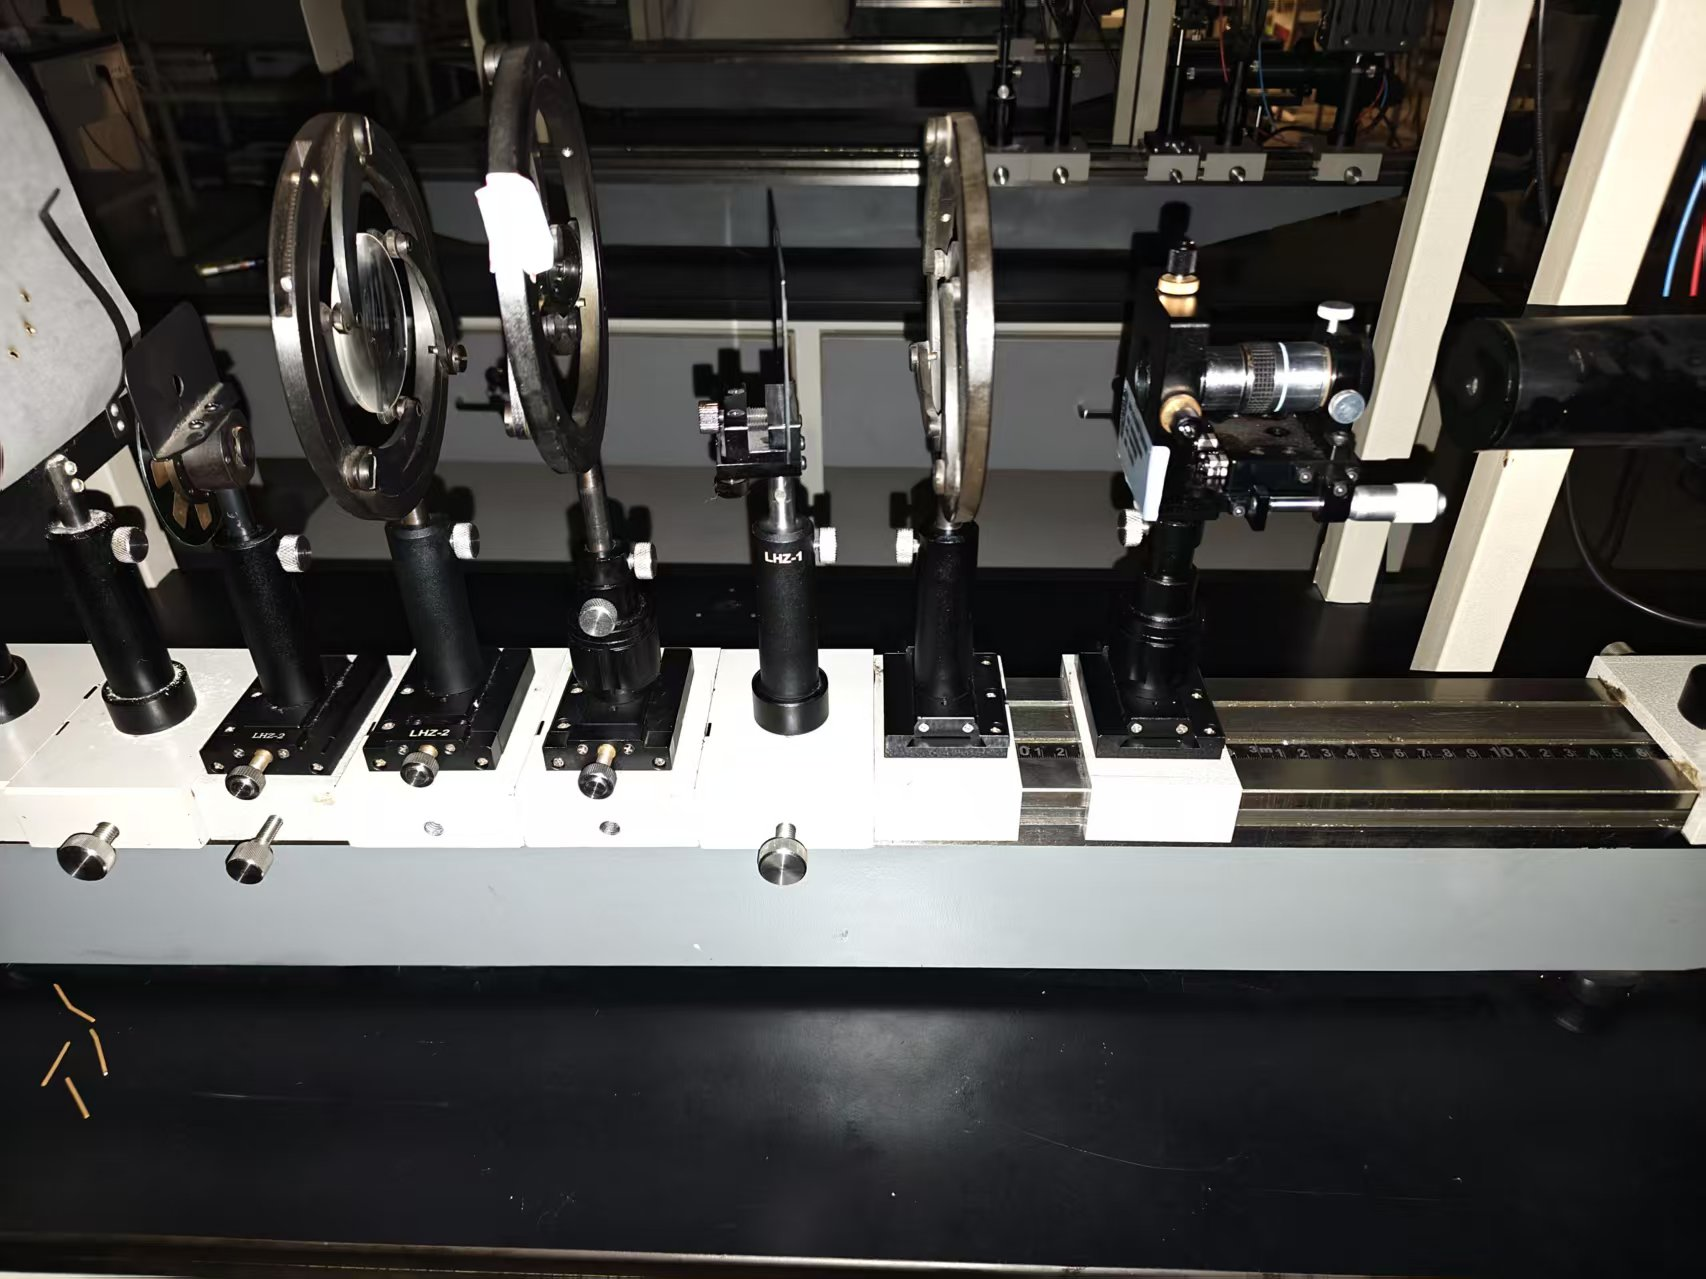
\includegraphics[width=0.7\textwidth]{fig0.jpg}
\end{figure}

\section{实验原理}
\subsection{傅里叶变换及在光学成象中的应用}
傅里叶光学中将物作为一个输入函数（物函数），研究它经过某种变
换后在接受面上将什么样的输出函数（象函数）。这样的分析方法与分
析线性电子网络相类似。如果物函数为 $g(x,y)$，可以将它可以表示成一
系列基函数 $\exp[\mathrm i 2\pi(f_xx+f_yy)]$ 的线性叠加

\begin{equation}
    g(x,y)=\iint_{-\infty}^{+\infty} G(f_x,f_y)\exp[\mathrm i2\pi(f_xx+f_yy)]\mathrm df_x\mathrm df_y
\end{equation}

其中，$f_x$ 和 $f_y$ 分别为在 $x$、$y$ 方向上的空间频率，即在单位长度内振
幅起伏的次数；$G(f_x, f_y)$ 被称为物函数 $g(x,y)$ 的空间频谱。空间频谱 $G( f_x,f_y )$
是这一叠加过程中，空间频率为 $f_x$、$f_y$ 的基函数的权重。它可以由物函
数 $g(x,y)$ 求得，其关系式为
\begin{equation}
    G(f_x,f_y)=\iint_{-\infty}^{+\infty} g(x,y)\exp[-\mathrm i2\pi(f_xx+f_yy)]\mathrm dx\mathrm dy
\end{equation}
实际上 $G(f_x,f_y)$ 和 $g(x,y)$ 描述的是同一光场，只是描述的角度不同。

理论和实验表明，一个完善的薄透镜是一个二维傅里叶变换运算
器，对于放置在物方焦面上物，在象方焦面上所成象就是物的傅里叶变
换，即在象方焦面上得到是物函数的频谱。对于焦距为 $F$ 的透镜，物函
数 $g(x,y)$ 放置在象方焦面 $x-y$ 平面，并以波长为 $\lambda$ 的相干光垂直照明，在
透镜的象方焦面 $\xi−\eta$ 面上得到 $g(x,y)$ 的傅里叶变换，即频谱
\begin{equation}
    G(\xi,\eta)=\iint_{-\infty}^{\infty}g(x,y)\exp\left[-\mathrm i \frac{2\pi}{\lambda F}(\xi x+\eta y) \right]\mathrm dx\mathrm dy
\end{equation}
空间频谱与坐标之间关系为
\begin{equation}
    f_x=\xi/\lambda F ,\quad f_y=\eta/\lambda F
\end{equation}

上面分析是对任意物函数进行的，对于在空间上具有周期性的物函
数，其空间频谱将是不连续的。式(3)也将由积分变成求和。即物函数可
以由一个傅里叶级数来表示。以一维二元光栅为例，它物函数可以表达
成
\begin{equation}
    g(x)=\begin{cases}
        1& nd-\frac b2\le x\le nd+\frac b2\\
        0& nd+\frac b2<x<(n+1)d-\frac{b}{2}
    \end{cases}
\end{equation}

这里 $g(x)$ 是振幅透过率，代表了光栅面上光场的分布形式，其中 $b$ 为透
光部分的宽度，$d$ 是光栅常数。将它的傅里叶级数表示为
\begin{equation}
    g(x)=G_0+\sum_{n=1}^\infty G_n \cos(2\pi n f_nx)
\end{equation}

式中 $f_n=n/d$，即光栅的第 $n$ 级空间频谱。当一个振幅为 $A$ 的平面波垂直
照射在光栅上，透过光栅的光，用它的频谱可表示为
\begin{equation}
    \begin{aligned}
        A=&A_0G_0+A_0\sum_{n=1}^{\infty}G_n\cos(2\pi nf_nx)\\
        =&A_0G_0+\frac{A_0}{2}\sum_{n=1}^{\infty}G_n[\exp(\mathrm i2\pi f_nx)+\exp(-\mathrm{i}2\pi f_nx)]
    \end{aligned}
\end{equation}
其中，$A_0G_0$ 是零级衍射光，$n$ 是衍射级次。方括号内第一项为正衍射级，
第二项为负衍射级。在空间频谱中它们分别为零频，正频和负频。 

\subsection{阿贝成像原理}

傅里叶变换在光学成象的重要性，首先是在研究显微镜成象中显示
出来。阿贝(E. Abbe)在1873年提出了显微镜的成象原理，这个理论不仅 
用傅里叶变换阐述了显微镜成象的机理，而更为重要的是首次引入频谱
概念和二次衍射成象的概念。阿贝成象原理认为，在相干光照明的情况
下，显微镜的成象可分为两个步骤；第一步通过物体的衍射光在物镜的
后焦面上形成一个初级衍射图（即频谱图），被称为次级光源；第二步
是这个次级光源所发出光经干涉叠加成为物镜的象平面的象。这个象可
以透过目镜观察到。

\subsection{光学空间滤波}
因为象（象函数）是由通过透镜的物函数各个付立叶分量重新组合
而成的，所以可以通过改变频谱函数，就可改变象函数。如果在透镜的
象方焦面，即在频谱面上人为地放置一些滤波器（吸收和项移）以该变
频谱面所需位置上的光振幅和位相，便可得到所需要的象函数。这个改
变频谱函数的过程就是空间滤波。最简单的滤波器就是一些特殊形状的
光阑，Figure 1 给出了几种常见的滤波器。低通滤波器可以阻挡住离光轴较
远的高频成分，让低频部分通过。可变光阑就属于这类滤波器。由于阻
挡了高频部分，象中失去了细节部分。高通滤波器则是阻挡低频部分，
让高频部分通过。如果滤去零频，则可除去图象中而背景，提高象的质
量。
\begin{figure}[H]
    \centering
    
\includegraphics[width=0.7\textwidth]{fig1.png}
    \caption{常见的振幅型空间滤波器}
\end{figure}

\subsection{实验内容}
1. 激光光束的准直扩束。按Figure 2 所示，利用显微镜物镜和一个透镜组
成一个望远镜，并将激光光束准直扩束。
\begin{figure}[H]
    \centering
    
\includegraphics[width=0.7\textwidth]{fig2.png}
    \caption{实验装置示意图}
\end{figure}

具体操作：依次调节激光器的俯仰与高度，显微镜的物镜的俯仰和高度，以及两个透镜的高度，使得光具组共轴，接受屏中央可以观察到光斑，且前后移动接受屏，光斑的中心几乎不发生移动。

2．空间滤波。用准直扩束后的激光光束照明网格字，适当调节透镜以及光屏位置，在频谱面上可以获得如 Figure 3 所示的频
谱。可以明显观察到频谱面上，形成了有规律的光点。
\begin{figure}[H]
    \centering
    
\includegraphics[width=0.4\textwidth]{fig3.png}
    \caption{频谱展开现象}
\end{figure}


(a)将接收屏放置在合适位置，观察“光”字的像。可以看到清晰的像，像中是一个一个小光点，说明横向和竖向的细节都得到保留。
\begin{figure}[H]
    \centering
    
\includegraphics[width=0.4\textwidth]{fig4.jpg}
    \caption{“光”字的像}
\end{figure}

(b)在频谱面上放置不同的滤波器，观察“光”字像的变化。

\begin{figure}[H]
    \centering
    \begin{subfigure}[b]{0.3\textwidth}
        \centering
        
\includegraphics[width=\textwidth]{fig5.jpg}
        \caption{竖向滤波器}
    \end{subfigure}
    \hfil
    \begin{subfigure}[b]{0.3\textwidth}
        \centering
        
\includegraphics[width=\textwidth]{fig6.jpg}
        \caption{横向滤波器}
    \end{subfigure}
    \hfil
    \begin{subfigure}[b]{0.3\textwidth}
        \centering
        
\includegraphics[width=\textwidth]{fig7.jpg}
        \caption{斜向滤波器}
    \end{subfigure}
    \caption{方向滤波器}
\end{figure}

对于方向滤波器，会使光保留对应方向的信息，丢失垂直方向的信息。放置竖向滤波器后，“光”字内出现竖向的条纹；放置横向滤波器后，“光”字内出现横向的条纹；放置斜向滤波器后，横向和竖向的信息都有保留，所以呈现的像与不放置滤波器几乎一样。

\begin{figure}[H]
    \centering
    
\includegraphics[width=0.4\textwidth]{fig8.jpg}
    \caption{低通滤波器}
\end{figure}

对于低通滤波器，阻挡了离光轴较远的高频部分，保留了低频部分，所以“光”字可以成象，但是内部的细节丢失掉了。

3．$\theta$ 调制。所谓 $\theta$ 调制就是利用不同取向的光栅调制物面上的不同部位。
如 Figure 7 所示的物面，天、地、房三个部分由三个不同取向的光栅进
行调制。三个光栅的取向之间各成120$\,^\circ$ 度角。实验步骤如下。

\begin{figure}[H]
    \centering
    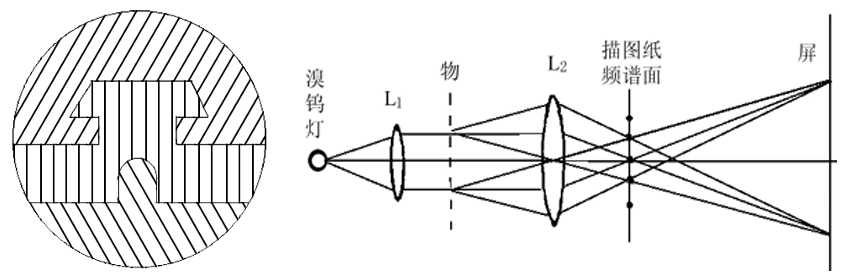
\includegraphics[width=0.8\textwidth]{fig8.png}
    \caption{$\theta$ 调制实验装置示意图}
\end{figure}

(a) 按 Figure 7 所示安排实验光路。用透镜 $L_1$ 将溴钨灯所发出的准直成平行
光，将物放置在平行光束中，移动 $L_2$ 将物清楚地成象在屏上。

(b) 将描图纸固定在毛屏上，移动其位置直至描图纸上接收到频
谱。

(c) 利用描图纸上的小孔，依次透过不同的频谱方向，确定好天、房子、草地所对应的频谱方向。

(d) 用支架固定描图纸，放至频谱接收位置，用一支点燃的香在
描图纸上烧出一些小孔，使对应地的绿光通过，对应房子的红光通过，
对应天的蓝光通过。屏上的象应为蓝天、绿地、红房子。
\begin{figure}[H]
    \centering
    
\includegraphics[width=0.4\textwidth]{fig10.png}
\end{figure} 

\section{思考题}

1.\textbf{傅里叶变换在光学成象系统的物理意义是什么？}

将物体的空间分布转化为频率域的空间频谱，从而允许从频率视角解析成像过程，其中各频率成分对应物体的特定结构特征，并为空间滤波技术奠定理论基础。

2.\textbf{利用阿贝原理，说明显微镜的分辨率受到什么因数限制？}

显微镜分辨率的限制因素源于阿贝原理，主要受透镜孔径和光波长的影响。透镜孔径决定了可透过的最高空间频率，孔径减小会导致高频成分减少，细节难以区分。同时，光波长增加会增大衍射角，使高频成分更难通过透镜，从而降低分辨率。

3.\textbf{何为频谱面，何为象面各在什么位置？}

频谱面是透镜的象方焦面，在此可以观察到物的频谱展开；象面是透镜成像后，物的象所在平面。

4.\textbf{什么是空间滤波？}

在频谱面放置滤波器，改变频谱的振幅或位相，从而改变象函数，其本质是对物的不同频率成分进行的人为选择。

5.\textbf{成象透镜的焦距为 $20\mathrm{cm}$ 正交光栅（铜网）的间距是 $0.1 \mathrm{mm}$，透明字的笔画粗 $1 \mathrm{mm}$。如果使象面上没有网格象，低通滤波器的孔径应该多大？}

物平面上的空间频率 $\nu$ 在透镜后焦平面上的径向坐标为
\begin{equation}
    x=f\lambda \nu
\end{equation}

在后焦面放一个圆形低通孔，直径为 $D$ ，它允许通过的最大空间频率为
\begin{equation}
    \nu_c=\frac{D}{2f\lambda}\quad \Rightarrow \quad D=2f\lambda\nu_c
\end{equation}

铜网网格对应的空间频率为
\begin{equation}
    \nu_g=\frac{1}{p}=10 \mathrm{mm^{-1}}
\end{equation}
透明字笔画对应的空间频率为
\begin{equation}
    \nu_w=\frac{1}{w}=1 \mathrm{mm^{-1}}
\end{equation}
要使得象面上没有网格象，空间频率 $\nu$ 应介于 $\nu_w \sim \nu_g$ 之间，所以孔径应该
\begin{equation}
    0.22 \mathrm{mm}=2f\lambda\nu_w<D<2f\lambda \nu_g=2.2\mathrm{mm}
\end{equation}

6.\textbf{阿贝成象原理是对显微镜的分辨率提出的，是否适用于其它光学成象系统？举例说明。}

阿贝成像原理不仅适用于显微镜，也适用于所有利用透镜成像的光学系统，例如，一个普通相机镜头的光圈越大图像越清晰；当光圈缩小时，分辨率下降并出现衍射模糊。这正是阿贝原理的体现，光圈限制了透镜能收集的空间频率范围，相当于在频谱平面上设置了一个低通滤波器。

7.\textbf{一个物体与周围介质的透明度是一样的，在正常的情况下，无法清楚地对它成象，这时采用那种空间滤波方式清楚地对它成象?}
采用相差滤波对其成象。过程为
\begin{itemize}
    \item (a)在透镜焦平面中，零级光集中在中心
    \item (b)在中心位置放一个 相环滤波片
    \item (c)相环对零级光引入$\pm90°$的相移
    \item (d)使零级光与衍射光干涉，把原本不可见的相位差变成亮度差,于是物体的位相结构变得清晰
\end{itemize}

\end{document}
